\documentclass[a4paper,11pt]{article}

\usepackage[margin=1.5cm]{geometry}
\usepackage[T1]{fontenc}
\usepackage[utf8]{inputenc}
\usepackage{lmodern}
\input{glyphtounicode}
\pdfgentounicode=1
\usepackage{microtype}
\DisableLigatures[f]{encoding = *, family = *}
\hyphenpenalty=10000
\exhyphenpenalty=10000
\tolerance=2000
\emergencystretch=3em

\usepackage{parskip}
\usepackage{xcolor}
\usepackage{graphicx}
\usepackage{tabularx}
\usepackage{titlesec}
\usepackage{enumitem}
\IfFileExists{fontawesome5.sty}{\usepackage{fontawesome5}}{%
  \newcommand{\faGlobe}{}\newcommand{\faEnvelope}{}%
  \newcommand{\faGithub}{github.com/}\newcommand{\faLinkedin}{linkedin.com/in/}}
\usepackage[unicode]{hyperref}

\definecolor{linkcolour}{rgb}{0.1,0.1,0.1}
\hypersetup{colorlinks,breaklinks,urlcolor=linkcolour,linkcolor=linkcolour,
  pdftitle={Adam Bekkar, CV},pdfauthor={Adam Bekkar}}

\titleformat{\section}{\Large\scshape\raggedright}{}{0em}{}[\titlerule]
\titlespacing{\section}{0pt}{10pt}{6pt}

\newenvironment{jobshort}[2]
{\noindent\begin{tabularx}{\linewidth}{@{}>{\raggedright\arraybackslash}X@{\hspace{1em}}>{\raggedleft\arraybackslash}p{4cm}@{}}
\textbf{#1} & #2
\end{tabularx}\\}
{\vspace{2pt}}

\pagestyle{empty}
\setlength{\parindent}{0pt}

\begin{document}

\noindent
\begin{minipage}[c]{0.72\textwidth}
 \raggedright
 {\LARGE\bfseries Adam Bekkar}\\[0.45em]
 {\small
 \faGlobe\ \href{https://adam.bekkar.ch}{adam.bekkar.ch}
 \ | \
 \faEnvelope\ \href{mailto:abekkar@student.ethz.ch}{abekkar@student.ethz.ch}
 \ | \
 \faGithub\ \href{https://github.com/Zeleph25}{Zeleph25}
 \ | \
 \faLinkedin\ \href{https://www.linkedin.com/in/adam-bekkar}{adam-bekkar}
 }\\[0.7em]
 Research interests: machine learning, probabilistic models, optimization, and computer systems.
\end{minipage}%
%\hfill
%\begin{minipage}[c]{3.7cm}
% \raggedleft
% 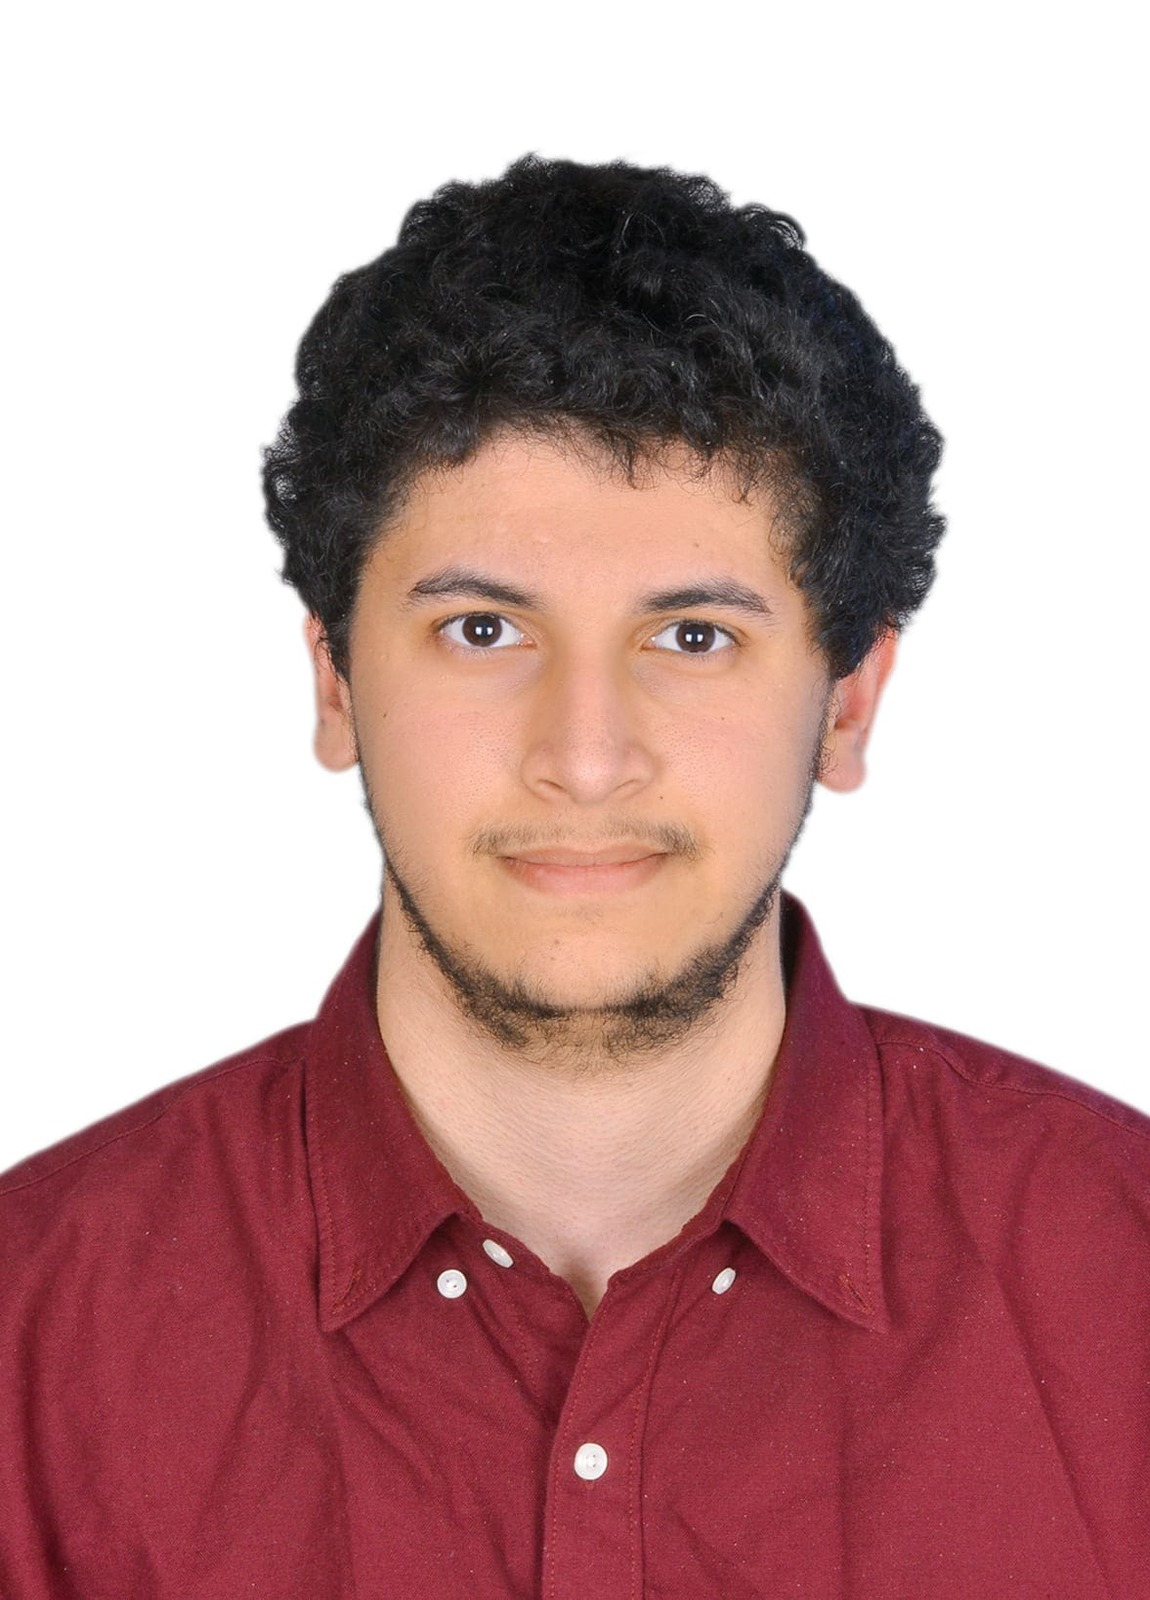
\includegraphics[height=4.4cm]{img/adam_bekkar.jpg}
%\end{minipage}

\vspace{0.6em}

\section{Education}
\begin{tabularx}{\linewidth}{@{}l X@{}}
2026 - Present & \textbf{ETH Zurich} - Master of Science in Computer Science. Major in Machine Intelligence, minor in Theoretical Computer Science. \par
\vspace{3pt}
Currently taking Advanced Machine Learning, Optimization for Data Science, Probabilistic Artificial Intelligence. \\[6pt]
2023 - 2026 & \textbf{\'Ecole Polytechnique F\'ed\'erale de Lausanne (EPFL)} - Bachelor of Science in Computer Science. Average: 5.1/6 \\[6pt]
2020 - 2023 & \textbf{Lyc\'ee Lyautey, Casablanca, Morocco} - French Baccalaureate with Highest Honours in Mathematics and Physics \\
\end{tabularx}

\section{Research}
\begin{jobshort}{\href{https://github.com/Zeleph25/polaris}{Polaris: Interactive Consistency under a Dishonest Majority}}{Sep 2026 - Present}
Research intern, DCL Lab, EPFL, with Prof. Rachid Guerraoui, supervised by Grigorii Emdin. Rust implementation of a protocol in which an elected leader broadcasts one verifiable vector instead of running $n$ parallel Byzantine broadcasts, measured against those baselines.
\end{jobshort}

\begin{jobshort}{\href{https://adam.bekkar.ch/papers/numalloc-cxl/}{NUMAlloc Evaluation on CXL-Enabled Hardware}}{Jun 2026 - Aug 2026}
Research intern, RS3 Lab, EPFL, with Prof. Sanidhya Kashyap, supervised by Musa \"Unal. Benchmarked NUMA allocators against jemalloc, tcmalloc, mimalloc, glibc, and others, and explored strategies to reduce latency across the CXL interconnect. \href{https://github.com/Zeleph25/cxl-alloc-benchmarks}{Scripts and results} on GitHub.
\end{jobshort}

\begin{jobshort}{\href{https://adam.bekkar.ch/papers/vnet/}{vNet: A Centrally Enforced Overlay Network for On-Site Programming Contests}}{Sep 2025 - Nov 2026}
Technical report on an overlay network in which every packet from a contestant machine is checked on organizer-controlled machines. \href{https://github.com/polympiads/vNet}{Code} and \href{https://github.com/polympiads/vNet-benchmarks}{benchmarks} on GitHub.
\end{jobshort}

\section{Teaching}
\begin{jobshort}{Student Assistant, Practice of Object-Oriented Programming (CS-108), EPFL}{Feb 2025 - Jul 2025}
Taught Java, object-oriented design, and core data structures in exercise sessions, and supported students on ReCHor, the semester-long project.
\end{jobshort}

\section{Projects}
\begin{jobshort}{\href{https://students4students.ch}{S4S-Connect - Students 4 Students}}{}
An app used by 1,000+ new students each year during EPFL's S4S integration week.
\end{jobshort}

\begin{jobshort}{\href{https://github.com/onepass-ch/onepass}{OnePass - Android Ticketing App}}{}
Team project for EPFL's Software Enterprise course (CS-311), built in Kotlin with a Firebase database. Placed 4th among 200+ students in the course's final contest, judged by a jury of CEOs.
\end{jobshort}

\section{Skills}
\vspace{2pt}
\noindent
\begin{minipage}[t]{0.30\linewidth}
\vspace{0pt}
\textbf{Languages}\\[8pt]
\begin{tabularx}{\linewidth}{@{}l @{\hspace{0.75em}} X@{}}
French  & Native \\[3pt]
Arabic  & Native \\[3pt]
English & C1 \\[3pt]
German  & Beginner
\end{tabularx}
\end{minipage}%
\hfill
\begin{minipage}[t]{0.66\linewidth}
\vspace{0pt}
\textbf{Skills}\\[8pt]
\begin{tabularx}{\linewidth}{@{}>{\bfseries}p{3.5cm} @{\hspace{0.8em}} >{\raggedright\arraybackslash}X@{}}
Languages & C, C++, Rust, Python, CUDA, SQL, Scala \\[3pt]
Parallel and HPC & CUDA, MPI, OpenMP, Slurm \\[3pt]
Systems & Docker, Kubernetes, gRPC, Linux, Grafana, CI, Git \\[3pt]
Hardware & Verilog, RISC-V
\end{tabularx}
\end{minipage}

\section{Leadership}
\begin{jobshort}{\href{https://students4students.ch}{President, Students 4 Students}}{Oct 2025 - Oct 2026}
Led an organizing team of twenty and coordinated more than a hundred staff for the week that prepares new students for EPFL.
\end{jobshort}

\begin{jobshort}{\href{https://students4students.ch}{Head of IT, Students 4 Students}}{Oct 2024 - Oct 2025}
Developed S4S-Connect, the web app the participants use during the integration week.
\end{jobshort}

\begin{jobshort}{Head of IT, Polympiads}{Sep 2025 - Aug 2026}
Built and maintained the distributed virtual network used for HC2 and Prologin, each hosting 300+ participants at EPFL.
\end{jobshort}

\begin{jobshort}{Class Representative, EPFL}{Sep 2025 - Jul 2026}
Represented students in discussions with faculty, collected feedback, and proposed improvements.
\end{jobshort}

\begin{jobshort}{IC Council Member, EPFL}{Sep 2025 - Jul 2026}
Represented students on the IC Faculty Council.
\end{jobshort}

\begin{jobshort}{\href{https://gitlab.com/agepoly/it/dev/trust}{IT Team Member, AGEPoly}}{Sep 2025 - Jul 2026}
Contributed to Trust, a rewrite of \texttt{truffe2.agepoly.ch}, the platform campus associations use to borrow equipment, book rooms, and manage accreditations.
\end{jobshort}

\end{document}